\documentclass[9pt,notes]{beamer}
%\documentclass{foils} %if wish to emulate the foils class using beamer

% - Style is ornate.

\mode<presentation>
{
%  \setbeamertemplate{background canvas}[vertical
%shading][bottom=red!10,top=blue!10]

    %% various themes available from the official Beamer user guide
    %\usetheme{default} %% blue, black, and white
    \usetheme{Madrid} %% red, white, and black
    %\usetheme{Frankfurt}
    \usefonttheme[onlysmall]{structurebold}
    %\usefonttheme[onlysmall]{structuresmallcapsserif}

    \setbeamercovered{transparent}
    % or whatever (possibly just delete it)
    %\usecolortheme{beetle}
}

\usepackage{multimedia}
\usepackage[english]{babel}
\usepackage{amsfonts, amsmath, mathrsfs}
\usepackage{amsxtra, amsthm, amssymb, amscd}
\usepackage{float}
\usepackage{graphics}
\usepackage{graphicx}
\usepackage{subcaption}
\usepackage{latexsym}
\usepackage{multimedia}
\usepackage{hyperref}
%\usepackage[dvips]{color} \usepackage{color}
%\usepackage{epsfig}
%\usepackage{mathrsfs}
%\usepackage{rotating}
%\usepackage{wrapfig}
%\usepackage[all]{xy}
%\usepackage{verbatim}

\setbeamercovered{dynamic}

\DeclareMathOperator*{\argmin}{arg\,min}
\DeclareMathOperator*{\argmax}{arg\,max}
\DeclareMathOperator{\Exp}{Exp}
\DeclareMathOperator{\grad}{grad}
\DeclareMathOperator{\Log}{Log}
\DeclareMathOperator*{\Cor}{Cor}
\DeclareMathOperator*{\diag}{diag}
\DeclareMathOperator*{\rank}{rank}
\DeclareMathOperator{\tr}{trace}


%%%% color-stuff, e.g., \Green{stuff you want to be printed in green}
\definecolor{LightGray}{rgb}{0.94,0.94,0.94}
\definecolor{VeryLightBlue}{rgb}{0.9,0.9,1}
\definecolor{LightBlue}{rgb}{0.8,0.8,1}
\definecolor{DarkBlue}{rgb}{0,0,0.6}
\definecolor{LightGreen}{rgb}{0.88,1,0.88}
\definecolor{MidGreen}{rgb}{0.6,1,0.6}
\definecolor{DarkGreen}{rgb}{0,0.6,0}
\definecolor{VeryLightYellow}{rgb}{1,1,0.9}
\definecolor{LightYellow}{rgb}{1,1,0.6}
\definecolor{MidYellow}{rgb}{1,1,0.5}
\definecolor{VeryLightRed}{rgb}{1,0.9,0.9}
\definecolor{LightRed}{rgb}{1,0.8,0.8}
\definecolor{Red}{rgb}{1,0,0}
\definecolor{Green}{rgb}{0,1,0}
\definecolor{Blue}{rgb}{0,0,1}
\definecolor{Gray}{rgb}{0.5,0.5,0.5}
\definecolor{Black}{rgb}{0,0,0}
\definecolor{White}{rgb}{1,1,1}
\newcommand{\White}[1]{{\color{White}{#1}}}
\newcommand{\VeryLightBlue}[1]{{\color{VeryLightBlue}{#1}}}
\newcommand{\LightBlue}[1]{{\color{LightBlue}{#1}}}
\newcommand{\DarkBlue}[1]{{\color{DarkBlue}{#1}}}
\newcommand{\DarkGreen}[1]{{\color{DarkGreen}{#1}}}
\newcommand{\VeryLightRed}[1]{{\color{VeryLightRed}{#1}}}
\newcommand{\LightRed}[1]{{\color{LightRed}{#1}}}
\newcommand{\Red}[1]{{\color{Red}{#1}}}
\newcommand{\Gray}[1]{{\color{Gray}{#1}}}
\newcommand{\Black}[1]{{\color{Black}{#1}}}
\newcommand{\Blue}[1]{{\color{Blue}{#1}}}
\newcommand{\Green}[1]{{\color{Green}{#1}}}
\newcommand{\LightGray}[1]{{\color{LightGray}{#1}}}


\newcommand{\R}{\mathbb{R}} % the standard 'set of all real numbers'
\newcommand{\N}{\mathbb{N}} % set of all natural numbers
\newcommand{\Z}{\mathbb{Z}} % integers
\newcommand{\Zpos}{\mathbb{Z}_{+}}
\newcommand{\image}{\mathrm{image}} % image of a function
\newcommand{\spn}{\mathrm{span}}
%
\newcommand{\Vmax}{\ensuremath{\mathcal{V}_{\max}}\xspace}
\newcommand{\Vargmax}{\ensuremath{\mathcal{V}_{\mathrm{argmax}}}\xspace}
\newcommand{\VSigma}{\ensuremath{\mathcal{V}_{\Sigma}}\xspace}
\newcommand{\Vsigma}{\ensuremath{\mathcal{V}_{\sigma}}\xspace}
\newcommand{\Sigmaneg}{\Sigma^{(-)}}	
%
\newcommand{\VSigmapos}{\ensuremath{\mathcal{V}_{\Sigma}^{(+)}}\xspace}
\newcommand{\VSigmaneg}{\ensuremath{\mathcal{V}_{\Sigma}^{(-)}}\xspace}
%
\newcommand{\Vmaxpos}{\ensuremath{\mathcal{V}^{(+)}_{\max}}\xspace}
\newcommand{\Vmaxneg}{\ensuremath{\mathcal{V}^{(-)}_{\max}}\xspace}
\newcommand{\alphapos}{\alpha^{(+)}}
\newcommand{\alphaneg}{\alpha^{(-)}}
\newcommand{\alphaiso}{\alpha_{{\tiny\textsc{ISO}}}}
%
%
\newcommand{\Hess}{\mathrm{Hess}} % fancy H for the hessian
\newcommand{\wein}{\mathsf{L}} % for the Weingarten map
\newcommand{\weinmat}{\widehat{\mathsf{L}}}
\newcommand{\img}{\mathtt{I}} % discrete image (a matrix, not the math term)
%
%%\DeclarePairedDelimiterX{\inner}[2]{\langle}{\rangle}{#1, #2}
%%\DeclarePairedDelimiterX{\vnorm}[1]{\Vert}{\Vert}{#1}
%%\DeclarePairedDelimiterX{\abs}[1]{\vert}{\vert}{#1}
%
%\newcommand{\bigO}{\mathcal{O}}
%
%\DeclareMathOperator{\FT}{\mathcal{F}} % fancy F for \FT
%\DeclareMathOperator{\DFT}{\mathcal{D}} % fancy D for \DFT

%%% theorem styles %%%%%%%%%
%\theoremstyle{plain}% default \newtheorem{thm}{Theorem}[section]
%\newtheorem{lem}{Lemma}[section]

%\theoremstyle{definition}
%\newtheorem{defn}{Definition}[section] \newtheorem{exmp}{Example}[section]
%\newtheorem{prop}{Proposition}[section] \newtheorem{cor}{Corollary}[section]

%\newtheorem{property}{Property}[section] \newtheorem{algorithm}{Algorithm}[section]

%\restylefloat{figure} \restylefloat{table}

%\usepackage[latin1]{inputenc} or whatever

\usepackage{beramono}

%\usepackage[T1]{fontenc}
% Or whatever. Note that the encoding and the font should match. If T1
% does not look nice, try deleting the line with the fontenc.

\beamertemplatenavigationsymbolsempty

\title[Cake Defense]{Optimized Strict Multiscale Frangi Prefiltering for Segmentation}
\subtitle{Towards an automated PCSVN extraction}

\author[{Luke Wukmer}] % (optional, use only with lots of authors)
{{Luke Wukmer}}%\inst{1}} \and S.~Another\inst{2}}
% - Use the \inst{?} command only if the authors have different
%   affiliation.

\institute[CSULB] % (optional, but mostly needed)
{
  %\inst{1}%
  Advisor: Dr. Jen-Mei Chang\\
  Department of Mathematics and Statistics\\
  California State University, Long Beach\\
  \texttt{lwukmer@gmail.com}
}
\graphicspath{{./figures/abstract_defense/}
              {./figures/abstract_defense/A-raw_targets/}
              {./figures/}
             }

\date{April 9, 2019}

\titlegraphic{
\includegraphics[height=2cm]{csulb-seal.png}}
\begin{document}

%%% TITLE SLIDE %%%%
\begin{frame} % % % % % % % % % % % % % % % % % % %
  \titlepage
\end{frame}

\section{Introduction}
\begin{frame} % % % % % % % % % % % % % % % % % % % % % % % % %
	\frametitle{Research Goals}
	\begin{columns}[c]
		\begin{column}{0.5\textwidth}
			\begin{figure}
			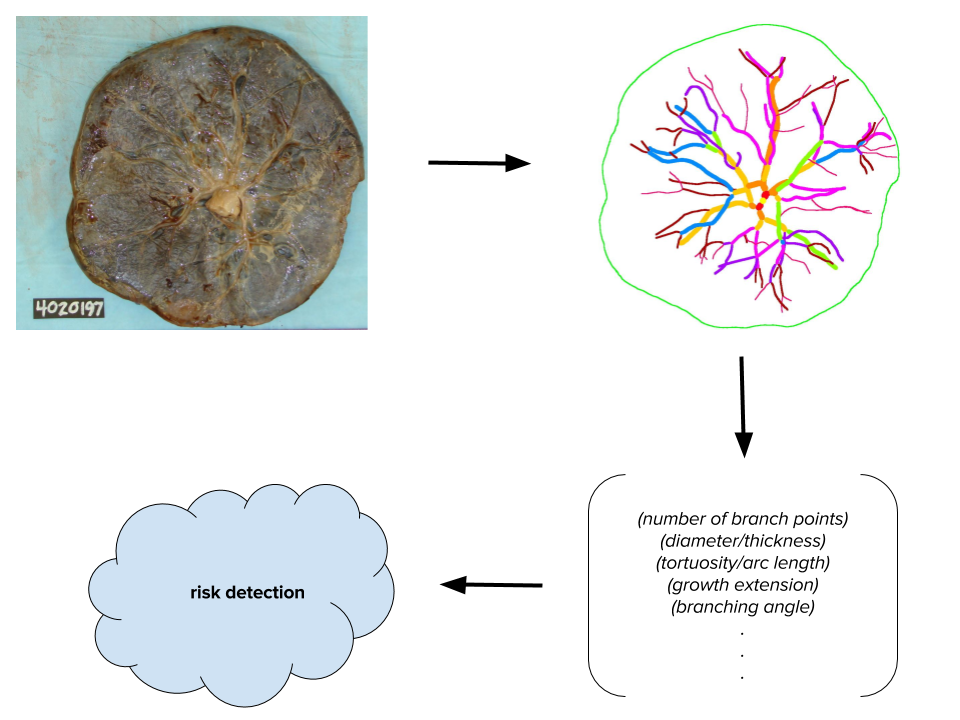
\includegraphics[width=\textwidth]{general_research_question.png}
			\note[item]{In the figure, a manual trace of the placental chorionic
            vascular surface network (PCSVN) is performed.
            This trace is measured in multiple ways. Those measurements are turned into
            a feature vector, which can be used to predict a risk. Refer to Boruta paper.}
			\end{figure}
		\end{column}
		\begin{column}{0.5\textwidth}
			\begin{block}{Vascular Network Extraction in Placentas}
				\begin{itemize}
					\item \textbf{Motivation:}
            Accurate measurement of the vascular structure of a placental sample
            can be used to predict neonatal risk factors, specifically ASD.
					\item \textbf{Challenge:}
						Currently no automated method of obtaining traces of
            PCSVN. Manual tracing is labor intensive but necessary
            for feature analysis.
            \note[item]{Manual tracing requires like 5 hours or something
                  and requires training.
                  There is some guesswork that's done in it too and some limitations
                  in the ground truth itself (will cover later)
                }
					\item \textbf{Research Goal:} Provide a fully automated method of extraction.
          					\end{itemize}
			\end{block}
		\end{column}
	\end{columns}
\end{frame}

\begin{frame}
  \frametitle{The Image Processing Problem}
  \begin{columns}[c]
  \begin{column}{0.5\textwidth}
    \begin{itemize}
        \begin{block}{Our image domain}
        \item The PCSVN is a connected network of veins and arteries
                on the surface of the placenta
        \item We have a ground truth for 201 samples
                from private NCS dataset
        \item Placentas have been formalin-fixed,
                so arteries are more prominent
                (there are issues)
        \item Pictures taken from top down, some glare,
                some inconsistencies.
        \item Placental images are comparatively noisy
        \note[item]{The surface of the placenta has a lot of changes
              in color/topology apart from the PCSVN
              so a lot of techniques that work elsewhere
              for vascular segmentation seem to fail here.
              Thus segmentation is more complicated that than say,
              an eyeball MRI (like original Frangi paper)
            }
      \end{block}
    \begin{block}{Strategy}
      Given the curvilinear nature of these vessels, we will appeal
      to differential geometry.
      \end{block}
    \end{itemize}
  \end{column}
  \begin{column}{0.5\textwidth}
    \centering
    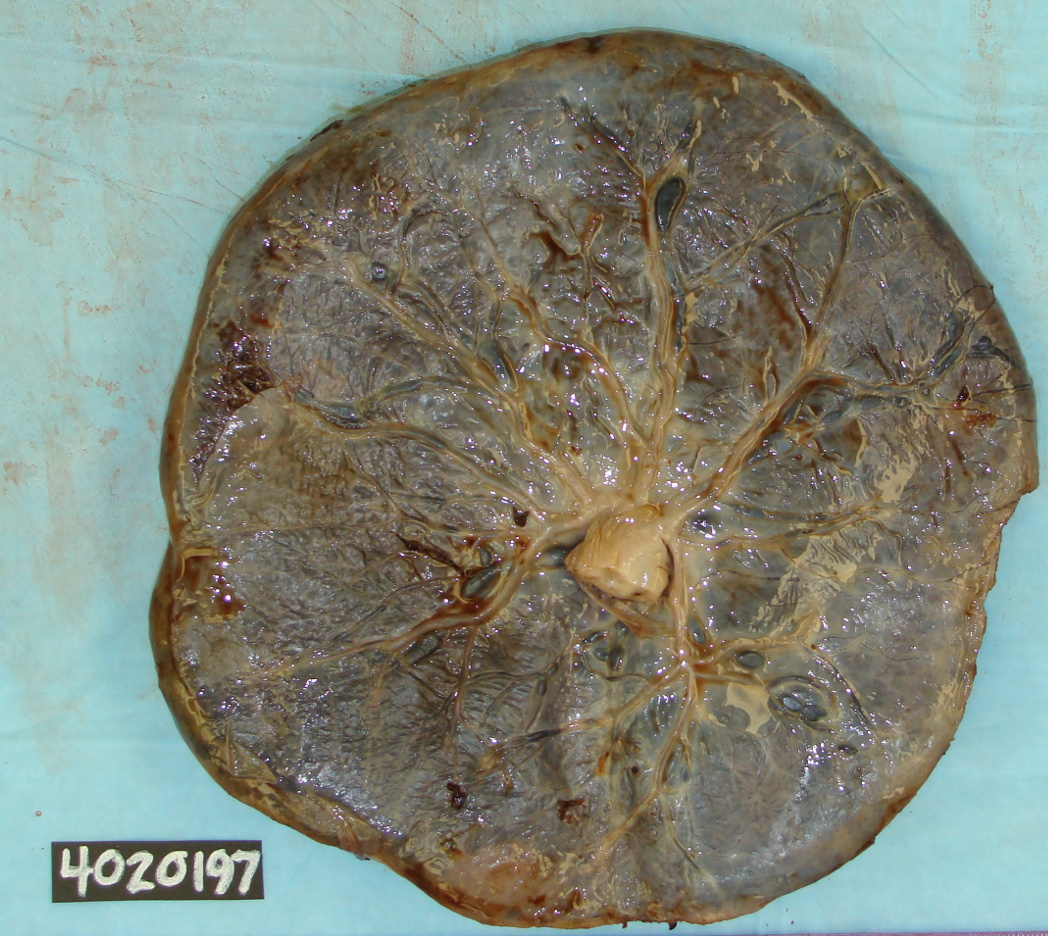
\includegraphics[height=0.36\textheight]{earli_crop.jpg} \\
    {\Huge $\Downarrow$}\\
    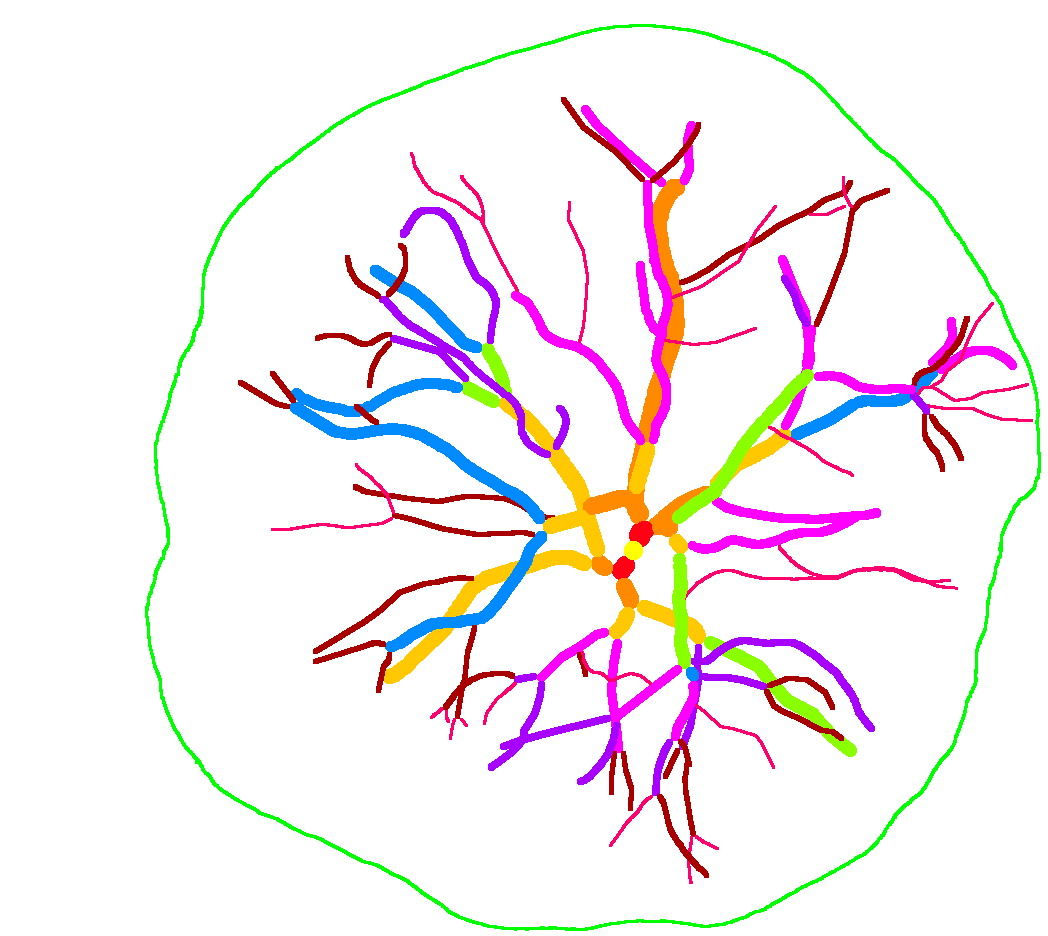
\includegraphics[height=0.36\textheight]{earli_crop_trace.jpg}
    \note[item]{Mention colors are simply vessel widths (3 to 19 odds)
          are part of the tracing protocol. that's really outside of the
          scope of this thesis, but kept anytime we show a ground truth
          because they're pretty
        }
    \note[item]{redo this page with a placenta from NCS, not EARLI}
  \end{column}
  \end{columns}
\end{frame}
%SLIDE 2/12 % % % % % % % % % % % % % % % % % % % % % % % % % % % % % % % % % % % % % % % %
%\begin{frame}
%	\frametitle{Previous Research}
%	
%	\begin{enumerate}[\bfseries(a)]
%	\item Nen Huynh used Frangi filtering result (different data set)
%	\item Frangi filtering is followed by morphological filtering (using principal-directions). Agreement with ground truth is displayed. 
%  \item There's a different research group using a cGAN or whatever and it's really good but
%    resource intensive, but whatever maybe just go with that one
%	\end{enumerate}
%	
%	\end{frame}


\section[Math Methods]{Mathematical Methods}
\begin{frame}
\frametitle{Appealing to Differential Geometry}
  Idealize image as a 3D surface (a graph) with $(x,y)$ spatial coordinates and intensity as the height function.
  \note[item]{Point of this slide is show that finding curvilinear surfaces is reasonable}

  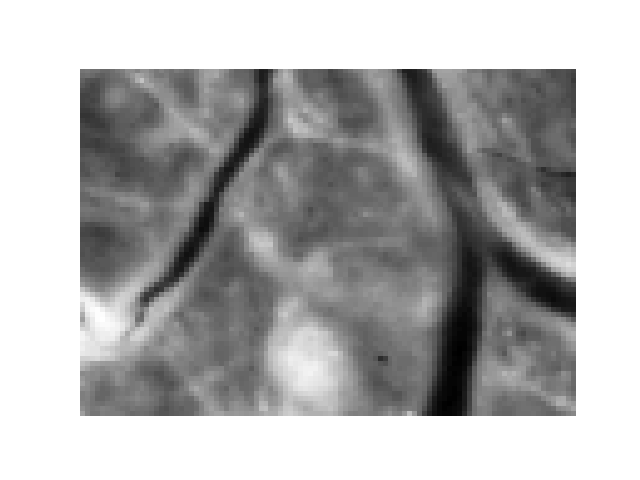
\includegraphics[width=0.3\textwidth]{inset_for_3d_surface}
  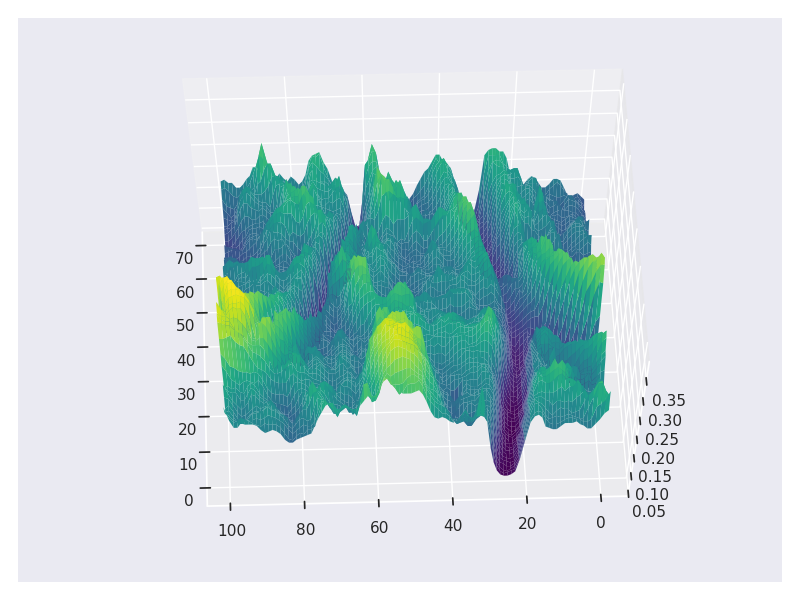
\includegraphics[width=0.6\textwidth]{inset_as_3d_surface}
  \note[item]{This point is a lot clearer when you show multiple vessel widths.}
  \note[item]{Also way clearer later when you show the surface after Gaussian blur,
  			  not sure if I should put that here and ``lie''/complicate things early on or not.}
  \note[item]{Crop graph, center, etc}
\end{frame}

\begin{frame}
\frametitle{Review of Differential Geometry of (Continuous) Surfaces}
\note[item]{``Let's just pretend we're dealing with this as a continuous surface
              for now''}
  \begin{itemize}
    \item (Thm of Meusnier)
          If you look at a point on the surface and fix a tangent vector,
          then all surface curves through that point with that velocity
          will have the same curvature there.
          So the curvature is intrinsic to the surface, call it normal curvature.
    \item Varying the tangent vector,
          we call extremal values of normal curvature the
          \textbf{principal curvatures}.
          The associated tangent vectors are \textbf{principal directions.}
    \item (Thm. of Olinde Rodrigues)
          These principal curvatures/directions are
          the eigenvalues/eigenvectors of
          a particular map called the \textbf{Weingarten map}.
      \note[item]{Weingarten map also called shape operator. Also can just define
                  the second fundamental form and use that matrix
                  (for our purposes)}
      \note[item]{Note that all this is true for \textit{any} kind of surface,
                  but we really just care about graphs.}
      \note[item]{If you want to get into notation, you can do so as far as explicitly
                  showing what the Weingarten map is (requires Gauss map).
                  You probably can avoid showing any setup of Meusnier--
                  defining curves and so on. 
                  }
  \end{itemize}
\end{frame}

\begin{frame}
\frametitle{Relationship Between Hessian and Weingarten Map for Graphs}
    \begin{block}{Weingarten Map for Graphs}
    Given the graph $f: U \to \mathbb{R}^3$ where $(x,y) \mapsto (x, y, h(x,y))$, the matrix
    representation of its Weingarten map is given by
    \begin{equation}
    \widehat{\mathsf{L}} = \mathrm{Hess}(h(x,y)) \tilde{G} \;,\quad \mathrm{where} \quad
    \tilde{G} := \frac{1}{\left({1+h_x^2 + h_y^2}\right)^{3/2}}
    \begin{bmatrix}
    1 + h_y^2 & -h_x h_y \\
    -h_x h_y & 1 + h_x^2 \\
    \end{bmatrix} 
    \end{equation}
    In particular, given a point $u = (x,y) \in U \subset \mathbb{R}^2$
    where $h_x \approx h_y \approx 0$, we
    have $\tilde{G} \approx \mathrm{Id}$, and thus
    $\widehat{\mathsf{L}} \approx \mathrm{Hess}(h)$.
  \end{block}
  \note[item]{Define hessian as the second derivative matrix}
  \note[item]{Make sure you have the graph definition clearly here. It's at the top but make it more prominent / earlier slidewise }
  \note[item]{Make point about when we're not at a critcial point, we don't guarantee
              any of this but it seems to work out okay}
  \note[item]{Fix notation in general}
  \begin{block}{Approximating}
    \begin{itemize}
    \item For ease of use, we can simply find eigenvalues of the Hessian instead.
    \item This gives rise to a class of filters, the so-called Hessian-based filters.
    \end{itemize}
    \end{block}
\end{frame}

\begin{frame}
  \frametitle{The Weingarten map and Principal Curvatures of a Cylindrical Ridge} 

Show the example here. Your example calculates from a different definition, like with Gauss map etc. so maybe rework or decide what you want here. 
\end{frame}


\section{The Frangi filter}
\begin{frame}
\frametitle{The (Uniscale) Frangi Filter}
\begin{gather*}
	\mathsf{H}(x,y) = \begin{bmatrix} h_{xx} & h_{xy} \\ h_{yx} & h_{yy} \end{bmatrix} \\
	\kappa_i , u_i \; \,\text{for}\; i=1,2
	\intertext{such that}
	\mathsf{H} u_i = \kappa_i u_i \;,\;
	\left|\kappa_1\right| < \left|\kappa_2\right|
\end{gather*}

Frangi filter definition here
\end{frame}

\begin{frame}
\frametitle[Anisotropy Factor]{Frangi filter anatomy: Anisotropy Factor}
\end{frame}

\begin{frame}
\frametitle[Structureness Factor]{Frangi filter anatomy: Structureness Factor}
\end{frame}

\begin{frame}
\frametitle[Frangi parameters]{Frangi filter anatomy: Choosing Parameters}
\begin{itemize}
\item Show the Frangi filter def. again.
\item Show a 3D graph of Frangi (just two, not 6x6 or whatever)
\item We will show a lot of data with different choices of parameters later.
\end{itemize}
\end{frame}

\begin{frame}
\frametitle[Scale Space Theory]{Scale Space Theory for Kids}
\begin{itemize}
  \item Obviously it's not actually a continuous surface
  \item Motivate and say some basic axioms
  \item Say convolution by gaussian solves these problems, derivatives work then too
\end{itemize}
\end{frame}

\begin{frame}
\frametitle{Implementation Detail: Calculating Discrete Hessian}
\begin{itemize}
  \item Calculate in frequency space
  \item Much much much faster
  \item Show the speed graph, explain MSE findings
\end{itemize}
\end{frame}

\begin{frame}
\frametitle{Frangi Filter Anatomy: Scale parameter}
\begin{itemize}
  \item Show scalewise outputs (inset)
  \item Describe relationship between vessel width and (LATER)
  \item Describe relative strength of outputs and what's too large (LATER)
  \item (Better to come back to these points later after describing research protocol)
\end{itemize}
\end{frame}

\begin{frame}
\frametitle{Multiscale Frangi filter}
\begin{itemize}
  \item Definition
  \item Standard Merging strategy
  \item It's faster so can pick more
  \item Logarithmic spacing is kind of sensible
  \item We can process each scale by itself too
\end{itemize}
\end{frame}


\section{Research Protocol}
\begin{frame}
\frametitle{The data set}
\end{frame}

\begin{frame}
\frametitle{Ground truth}
\end{frame}

\begin{frame}
\frametitle{Imperfections/Complications in Data set}
\end{frame}

\begin{frame}
\frametitle{Preprocessing: Glare}
\end{frame}

\begin{frame}
\frametitle{Preprocessing: Umbilical Stump}
\end{frame}

\section{Analysis (Pre-segmentation)}

\begin{frame}
\frametitle{Cumulative Vesselness Ratio}
Just show a few parametrization methods, don't show all
\end{frame}

\section{Frangi Segmentation Methods}
\begin{frame}
\frametitle{Fixed threshold of Vmax}
\end{frame}

\begin{frame}
\frametitle{Scalewise percentile filtering}
\end{frame}

\begin{frame}
\frametitle{Trough-filling (1/2)}
Show definition of signed Frangi, inset
\end{frame}

\begin{frame}
\frametitle{Trough-filling (2/2)}
\end{frame}

\begin{frame}
\frametitle{A non-Frangi segmentation method: ISODATA}
This represents a good idea that doesn't rely on diffgeo or local anything
\end{frame}

\section{Frangi Segmentation Results}
\begin{frame}
\frametitle{Binary Classification (1/2)}
Confusion matrix with TP, FP, TN, FN
\end{frame}

\begin{frame}
\frametitle{Binary Classification (2/2)}
MCC and Precision Scores
\end{frame}

\begin{frame}
\frametitle{Example Segmentation Results}
Spend a couple slides here talking about
\begin{itemize}
  \item parametrization choices effect
  \item threshold choices effect
  \item talk about ``good'' false positives and  ``bad'' false positives
  \item talk about good samples and bad samples
\end{itemize}
\end{frame}

\begin{frame}
\frametitle{Boxplots}
\end{frame}

\begin{frame}
\frametitle{Conclusion}
\end{frame}

\begin{frame}
\frametitle{Appendix}
Put some proofs / extra things here
\end{frame}

\end{document}